\section{Analisi}
\subsection{Requisiti}

Il progetto si pone l'obiettivo di ricreare il gioco da tavolo "Carcassone" 1 ispirandosi anche alla sua controparte videoludica 2. Il gioco consiste in un posizionamento tessere a turni, da 2 a 6 giocatori, in cui l’obiettivo di ogni giocatore è quello di accumulare più entro la fine della partita. Ogni tessera ha quattro lati e raffigura una particolare parte di mappa composta da strade, città, campi e monasteri e deve essere posizionata adiacentemente ad almeno un lato identico di un'altra tessera. La meccanica principale del gioco è quella di “chiudere” le strutture come raffigurato nelle figure 1 e 2 e 3 con al loro interno un seguace del proprio colore.

\begin{figure}[]
    {\includegraphics[]{images/Città.png}}

    \caption{chiudere una città comporta l’assenza di parti non murate per un totale di 2 punti per ogni tessera, aggiungendo 2 per ogni tessera con lo stemma}
\end{figure}

\begin{figure}[]
    {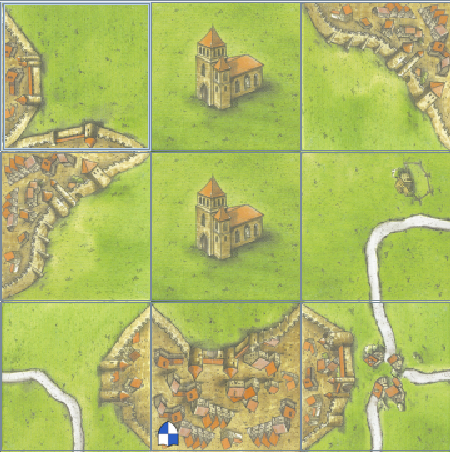
\includegraphics[]{images/Monastero.png}}

    \caption{chiudere un monastero comporta la presenza di tutte e 8 le tessere a circondarlo a circondarlo per un totale di 9 punti}
\end{figure}

\begin{figure}[]
    {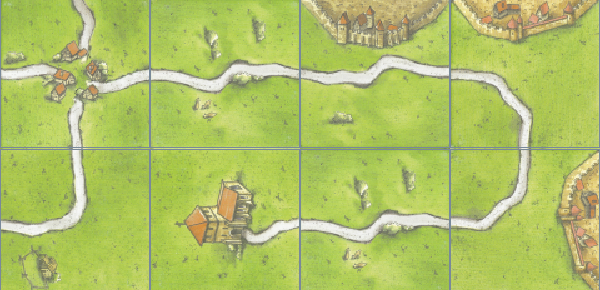
\includegraphics[]{images/Strada.png}}

    \caption{chiudere una strada comporta la presenza di un incrocio o un un’entrata ad un monastero o città da ambo i lati per un totale di 1 punto per ogni tessera, estremi compresi}
\end{figure}

\subsection*{Requisiti funzionali}

\begin{itemize}
\item Calcolo del punteggio progressivo: ogni giocatore avrà il suo punteggio corrente che incrementerà ogni volta che durante il suo turo "chiuderà" una struttura seguendo le regole del gioco
\end{itemize}

\begin{itemize}
\item Calcolo del punteggio al termine del gioco: ogni giocatore otterrà il suo punteggio finale sommando al suo punteggio corrente il punteggio ogni seguace ancora presente nel terreno quindi

\subitem i punteggi residui di ogni seguace posizionato in una struttura non "chiusa"

\subitem i punteggi ottenuti da ogni seguace posizionato in un prato seguendo le regole del gioco come nella figura 4

\begin{figure}[]
    %{\includegraphics[]{images/Prato.png}}

    \caption{Ogni prato è delimitato e rappresentato da ogni strada e città che lo circonda}
    
    % , ed è rappresentato dall'insieme di ogni tessera
    % Un prato è rappresentato dall'insieme di ogni sezione verde presente sulle tessere che ne delimitano i lati tramite strade e città}
\end{figure}

\end{itemize}
\begin{itemize}
\item Menù principale, con selezione numero giocatori
\end{itemize}
\begin{itemize}
\item Gestione turno del giocatore
\end{itemize}
\begin{itemize}
\item Gestione posizionamento pedine
\end{itemize}
\begin{itemize}
\item Calcolo delle posizioni valide per le tessere: ad ogni tentativo di posizionamento della tessera dovrà essere verificata la possibilità di effettuare l'azione. Si gestirà anche il caso in cui la tessera dovrà esssere obbligatoriamente scartata in quanto non esistono posti validi in cui in cui posizionarla
\end{itemize}
\begin{itemize}
\item Gestione della creazione o ampliamento di prati, città e strade
\end{itemize}

\subsection*{Requisiti non funzionali}
\begin{itemize}
\item Menù di pausa e salvataggio sessione
\end{itemize}
\begin{itemize}
\item Possibilità di visualizzare le tessere rimanenti
\end{itemize}
\begin{itemize}
\item Scelta del colore dell’avatar
\end{itemize}
\begin{itemize}
\item Gestione dell’audio
\end{itemize}
\begin{itemize}
\item Aggiunta di espansioni del gioco (nuove tessere e regole modificate)
\end{itemize}
\begin{itemize}
\item Sviluppo di una semplice AI per permettere una modalità singleplayer
\end{itemize}

\subsection{Analisi e modello del dominio}
L'analisi e il modello di dominio di Carcassonne possono essere suddivisi in diversi componenti chiave, tra cui il tabellone di gioco, le tessere, i meeples e il sistema di punteggio.
\begin{itemize}
    \item Tabellone di gioco (Mappa): Il tabellone di Carcassonne rappresenta la regione di Carcassonne ed è composto da una serie di tessere che vengono posizionate sul tabellone durante il gioco. Il tabellone è suddiviso in diverse regioni, tra cui città, strade, campi e monasteri. Ognuna di queste regioni ha le proprie regole e il proprio sistema di punteggio, che aggiungono profondità e complessità al gioco.
    \item Le tessere (Tiles): Le tessere di Carcassonne rappresentano diversi tipi di terreno, tra cui città, strade, campi e monasteri. Queste tessere vengono estratte casualmente da una pila e devono essere posizionate sul tabellone di gioco in modo che corrispondano al tipo di terreno delle tessere circostanti. Ogni tessera ha le sue regole e il suo sistema di punteggio, che i giocatori devono seguire per massimizzare i loro punti.
    \item Meeples: I meeple sono i pezzi di gioco che i giocatori usano per controllare le diverse regioni del tabellone. 
    \item Sistema di punteggio: Il sistema di punteggio di Carcassonne si basa sul completamento di diverse regioni sul tabellone di gioco. Quando una città, una strada o un monastero vengono completati, il giocatore che ha il maggior numero di meeples su di essi ottiene i punti. Se più giocatori hanno meeples su un elemento completato, ognuno di loro ottiene i punti. Alla fine della partita, i giocatori ottengono punti anche per i loro contadini sui campi completati. Il giocatore con il maggior numero di punti alla fine del gioco è il vincitore.
\end{itemize}
Le difficoltà che il progetto mantiene sono sopratutto presenti nella parte grafica, non ancora ottimizzata a causa dell'utilizzo del framework grafico Java Swing.
